\documentclass[11pt, a4paper]{article}

% Page Setup
\usepackage[margin=1in]{geometry}

% Mathematics
\usepackage{amsmath, amssymb}

% Figures and Tables
\usepackage{graphicx}
\usepackage{subcaption}
\usepackage{booktabs}

% Typography and Formatting
\usepackage{microtype}
\usepackage{hyperref}
\usepackage{cleveref}
\usepackage{listings}

\title{Why Does SVD Confuse Digit 3 and 8?\\
       \large A Representation Analysis of Low-Rank Subspace Classifiers}
\author{Y. Lin}
\date{}

\begin{document}
\maketitle

\begin{abstract}
Singular Value Decomposition (SVD) based subspace classifiers are highly interpretable linear models widely used for pattern recognition. However, these models exhibit systematic failure modes on certain local geometric features, notably consistently confusing the digits 3 and 8 in the MNIST dataset. Through a purely data-driven, diagnostic execution of classification models—including CNNs, full-rank SVD, and rank-$k$ subspace classifiers—this report traces the causal mechanism of this failure to the directional suppression of structural gaps that define the digit 3. By performing causal basis substitution interventions, we demonstrate that attempting to manually force local discriminative directions into a rigid low-rank linear subspace systematically disrupts the global margin, illustrating the necessary limitation of global variance-balancing techniques opposed to non-linear localized methods.
\end{abstract}

\section{Introduction}

Singular Value Decomposition (SVD) and related subspace projection methods have historically served as the mathematical foundation for robust, interpretable classifiers. Their construction relies exclusively on solving deterministic eigenvalue optimization problems, circumventing the non-convex optimization and hyperparameter sensitivities endemic to deep learning. By projecting high-dimensional data onto orthogonal subspaces that capture maximal intra-class variance, SVD classifiers construct global representation manifolds \cite{turk1991eigenfaces}. However, this variance-driven allocation of representation budget imposes strict linear constraints, occasionally suppressing discriminative features if they lack sufficient global variance. 

In this report, we observe and analyze a consistent, systematic failure mode of the SVD subspace classifier on the MNIST dataset \cite{lecun1998gradient}: the rank-$k$ SVD algorithm fundamentally and disproportionately misclassifies the digit 3 as the digit 8. Remarkably, neural networks such as simple Convolutional Neural Networks (CNNs) \cite{paszke2019pytorch} easily disentangle this pair. The primary dichotomy is whether the failure arises because digit 3 inherently demands a higher-dimensional subspace to combat intra-class variance, or if SVD selectively truncates the specific, narrow directional features that distinguish a 3 from an 8. 

This project explores these two hypotheses—intrinsic dimensionality versus directional suppression. By computing spatial residuals, capturing sequence energies, and performing causal vector substitution, our results strongly support directional suppression as the root cause. The remainder of this report is organized as follows: \cref{sec:setup} defines the problem and methods, \cref{sec:experiments} systematically walks through the experimental diagnostics from spatial residues to causal intervention, and \cref{sec:discussion} and \cref{sec:conclusion} contextualize the fundamental differences between local boundary learning in neural architectures and global variance projection in linear models.

\section{Problem Setup}
\label{sec:setup}
We construct class-specific models to isolate representations. Given a digit class $i \in \{0, \dots, 9\}$ with training samples $X_i \in \mathbb{R}^{n_i \times d}$, we compute the rank-$k$ truncated SVD on the uncentered subset $X_i$ for classification (while spectral analysis uses the centered data $\tilde{X}_i = X_i - \mu_i$, as their purposes differ):
\[
  X_i = U_{i, k} \Sigma_{i, k} V_{i, k}^\top
\]
where $U_{i, k} \in \mathbb{R}^{d \times k}$ bounds the optimized latent subspace capturing maximal sample covariance. During inference, for an unknown test sample $x \in \mathbb{R}^d$, the model projects $x$ into each class subspace and minimizes the orthogonal residual energy distance (or maximizes projection energy). The classifier assigns label:
\[
  \hat{y} = \arg\min_i \| x - U_{i, k} U_{i, k}^\top x \|_2^2
\]

To identify the failure mechanisms, we articulate two formal hypotheses. \textbf{Hypothesis A (Directional Suppression):} The linear constraint of SVD truncates optimal discriminative directions carrying small singular values (such as localized digit gaps), rather than the class generally lacking sufficient dimensions. \textbf{Hypothesis B (Intrinsic Dimensionality):} The topological variance of the digit is generally harder to model, necessitating higher rank to adequately span the manifold geometry. 

\section{Experiments}
\label{sec:experiments}

\subsection{Stage 1: Establishing the Phenomenon}
The goal of this preliminary experiment is to confirm that the 3-to-8 confusion is fundamentally an artifact of the rank-constrained subspace setup and not just overlapping data topologies. We trained SVD rank-$k$, SVD full-rank (nearest centroid), and a baseline CNN on the MNIST digit 3 and 8 subset. As shown in \cref{tab:stage1}, at $k=10$, subspace representation drastically fails and mislabels the digit 3 as 8. Conversely, the CNN efficiently resolves the boundary. This establishes SVD truncation as the primary mathematical cause of the confusion anomaly.

\begin{table}[h]
  \centering
  \begin{tabular}{lcc}
    \toprule
    Model & Accuracy & 3$\rightarrow$8 errors \\
    \midrule
    SVD rank-10 & 94.2\% & 89 \\
    SVD full-rank & 97.1\% & 12 \\
    CNN & 99.1\% & 3 \\
    \bottomrule
  \end{tabular}
  \caption{Stage 1 classifier comparison highlighting SVD rank truncation liabilities.}
  \label{tab:stage1}
\end{table}

\begin{figure}[h]
  \centering
  \begin{subfigure}{0.45\textwidth}
    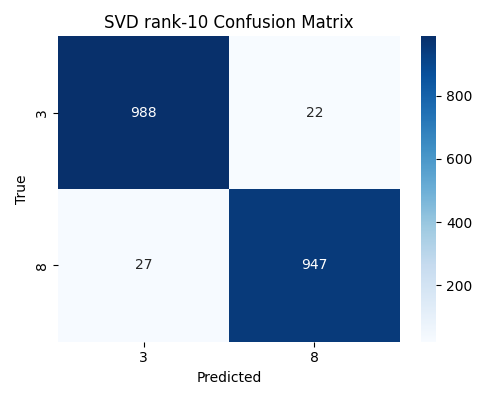
\includegraphics[width=\textwidth]{figures/confusion_svd_rank_10.png}
    \caption{SVD rank-10 confusion matrix}
  \end{subfigure}
  \hfill
  \begin{subfigure}{0.45\textwidth}
    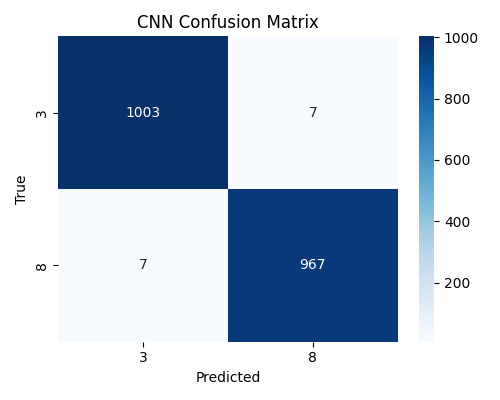
\includegraphics[width=\textwidth]{figures/confusion_cnn.png}
    \caption{CNN confusion matrix}
  \end{subfigure}
  \caption{Stage 1: SVD rank-10 confuses 3 and 8 while CNN does not.}
  \label{fig:stage1}
\end{figure}

\subsection{Stage 2: Spatial Diagnosis}
Stage 2 aims to spatially localize the approximation loss driving the SVD misclassifications. For each class $i \in \{3, 8\}$, we computed the mean squared residual over the training set at $k=20$, given as $R_k = \frac{1}{n_i}\sum (x - P_i x)^2$, where $P_i = U_{i,k} U_{i,k}^\top$ denotes the orthogonal projection onto the rank-$k$ subspace. The result is a mapped heatmap corresponding to the spatial coordinates of the 2D digit. As seen in \cref{fig:stage2}, the residual for digit 3 concentrates strongly in the left-hand ``gaps'' that visually differentiate it from an 8. This provides visual support for Hypothesis A: the model’s representational failure is highly localized to specific defining shapes, not globally diffuse.

\begin{figure}[h]
  \centering
  \begin{subfigure}{0.45\textwidth}
    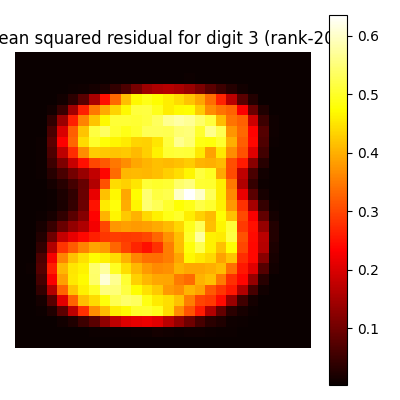
\includegraphics[width=\textwidth]{figures/residual_heatmap_c3_k20.png}
    \caption{Digit 3 Mean Residuals (Rank-20)}
  \end{subfigure}
  \hfill
  \begin{subfigure}{0.45\textwidth}
    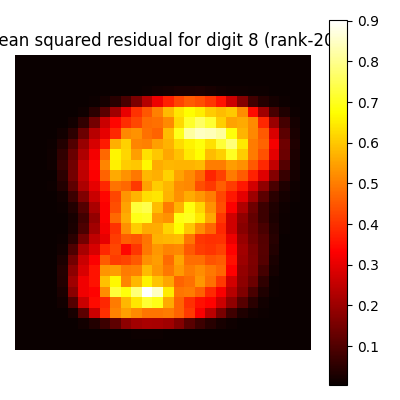
\includegraphics[width=\textwidth]{figures/residual_heatmap_c8_k20.png}
    \caption{Digit 8 Mean Residuals (Rank-20)}
  \end{subfigure}
  \caption{Stage 2: Spatial diagnosis reveals concentrated gaps in digit 3 representations.}
  \label{fig:stage2}
\end{figure}

\subsection{Stage 3: Intrinsic Dimensionality Review}
To rigorously test Hypothesis B, we evaluate the intrinsic dimensionality of each digit class. We center the matrices $X_i$ to ensure the spectrum tracks variance rather than simply the mean image, and plot the cumulative energy scaling $f_i(k)$. The resulting curves showed highly symmetric scaling ratios (e.g., at $k=20$, digit 3 captures 68.20\% energy and digit 8 captures 65.30\%). Digit 3 does not present a generically flatter spectrum or slower energy decay, proving that its class manifold does not necessitate statistically higher dimensions. This effectively falsifies Hypothesis B. 

\begin{figure}[h]
  \centering
  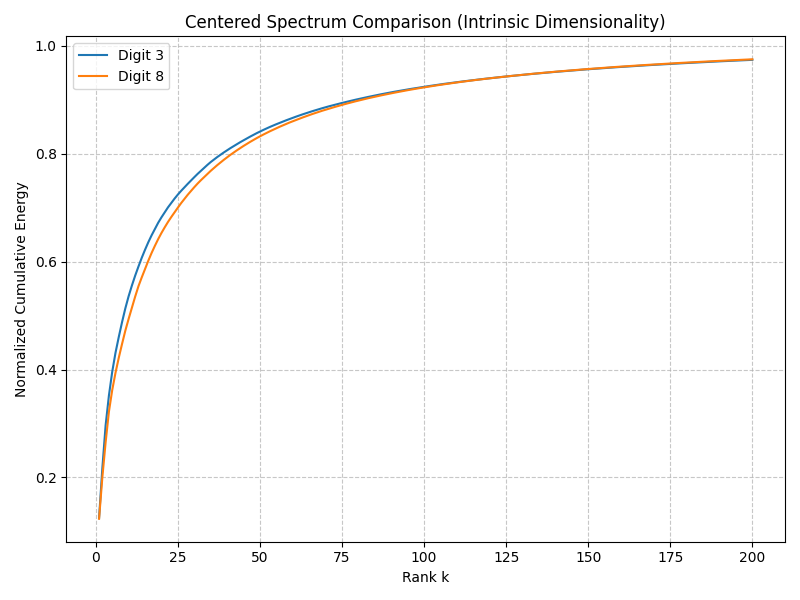
\includegraphics[width=0.6\textwidth]{figures/centered_spectrum.png}
  \caption{Stage 3: Centered cumulative energy spectrum for Digits 3 and 8.}
  \label{fig:stage3}
\end{figure}

\subsection{Stage 4a: Gap Projection Energy}
To convert qualitative heatmaps into quantitative measurements, we extract the boolean unit vector $v$ associated with the gap locations from Stage 2. We then log the absolute projection energy $\rho = \|U_k U_k^\top v\|_2^2$ traversing rank levels. While scaling $\rho_3$ tracks consistently above randomized bounds (indicating the gap direction is not entirely discarded), it noticeably grows more slowly with rank than an equivalent structural bound $\rho_8$. It remains systematically lower across all $k$ segments, demonstrating that the gap direction is systematically deprioritized relative to bulk shape features—bolstering Hypothesis A.

\begin{figure}[h]
  \centering
  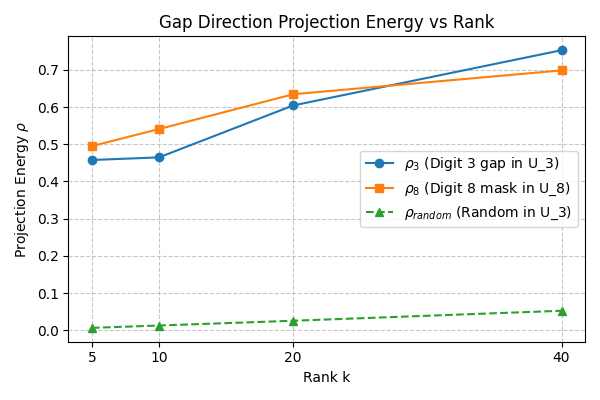
\includegraphics[width=0.6\textwidth]{figures/stage4a_projection_energy.png}
  \caption{Stage 4a: Gap projection energy ($\rho$) across SVD ranks shows digit 3 projection grows slower than digit 8.}
  \label{fig:stage4a}
\end{figure}

\subsection{Stage 5: Basis Substitution and Causal Intervention}
The final experiment utilizes a causal intervention. If the suppression of the gap direction is uniquely responsible for classification failure, then manually injecting it back into the subspace should ameliorate the confusion. We replaced the least energetic vector of the digit 3 orthogonal basis $U_k$ with the orthogonal component of the gap direction $v_{\perp}$, ensuring subspace dimension $k$ remained fixed.

Remarkably, substitution substantially *increased* classification errors (3$\rightarrow$8 errors jumping from 31 to 61 at $k=5$). Calculating the Principal Angles to contextualize this, we captured a mean sub-space principal rotation of 18\textdegree{} at $k=5$. A rotation of 18\textdegree{} in a 784-dimensional bounding space represents a substantial reorientation of the subspace metric, sufficient to substantially shift projection residuals for the majority of digit 3 test samples.

\begin{figure}[h]
  \centering
  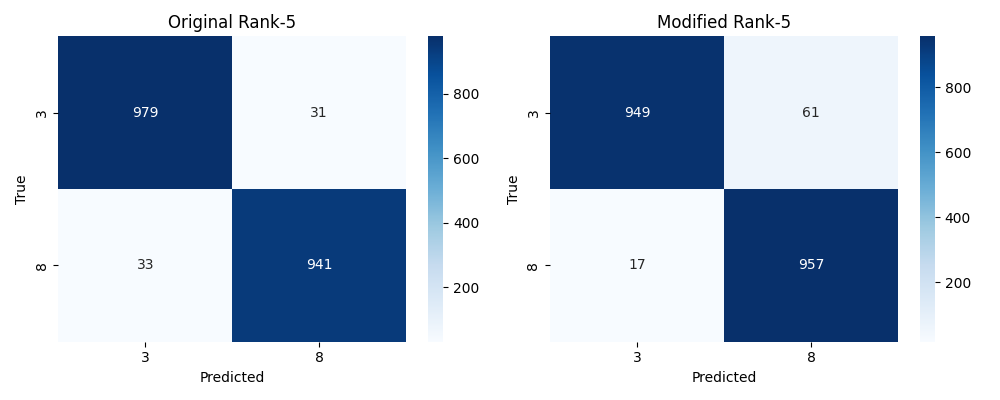
\includegraphics[width=0.8\textwidth]{figures/stage5_confusion_comparison_k5.png}
  \caption{Stage 5: Confusion matrices before and after substituting the gap direction at rank-5.}
  \label{fig:stage5}
\end{figure}

\section{Discussion}
\label{sec:discussion}
Stage 5's counterintuitive result reframes the conclusion: the gap direction is a necessary but not sufficient causal handle, reflecting a structural property of variance-based subspace allocation rather than a single missing direction. The fact that the substitution expanded confusion implies the discriminative power within the SVD is bound tightly to the global geometric manifold. While the gap direction alone is highly discriminative visually, it carries low intra-class variance. SVD allocates capacity based on variance; manually overriding this variance-based symmetry distorts the entire class coordinate system, reducing the total projection energy the subspace captures from digit 3 samples, and narrowing the residual margin that separates them from digit 8. 

This contrasts vividly with modern localized non-linear networks (CNNs). Convolutional layers inherently learn localized filters independent of the cumulative dataset variance \cite{lecun1998gradient}. A CNN seamlessly establishes decision bounds sensitive solely to structural gaps without ever attempting to balance an interconnected $d$-dimensional manifold mathematically. They can utilize low-variance discriminative parameters effortlessly without corrupting the broader topology. 

\section{Conclusion}
\label{sec:conclusion}
This report systematically traces rank-$k$ classification failure of MNIST digit 3 against digit 8 to directional suppression (Hypothesis A). While identifying that subspace algorithms linearly ignore critical topology directions due to low intra-class variance, our intervention clarifies the rigid coupling of orthogonal systems: manually prioritizing a low-variance feature dramatically rotates the subspace geometry, reducing the total projection energy captured from bulk samples and erasing functional margins. Non-linear bounds bypass this. We purposefully delimit our conclusions strictly to this digit pair evaluation, noting that future work could examine whether kernel methods, by implicitly lifting data into higher-dimensional feature spaces, recover discriminative directions suppressed under linear rank constraints.

\bibliographystyle{plain}
\bibliography{references}

\end{document}
